\documentclass{article}
\usepackage[margin=0.5in]{geometry}
\usepackage{graphicx}
\usepackage{wrapfig}
\usepackage{amsmath}
\graphicspath{{Images/}}
\usepackage[ampersand]{easylist}

\usepackage{natbib}
\bibliographystyle{abbrvnat}
\setcitestyle{authoryear,open={(},close={)}}

\begin{document}
	
\title{Single Camera Autonomous Vehicle Navigation Localisation Implementation Discussion}
\author{Michael McDonnell}
\date{}
\maketitle

\section{Overview}
During the course of development of the single camera autonomous vehicle navigation localisation system, several implementation points were identified. These points were deemed outside the scope of discussion in the original article however are included here in an effort to preserve the information. This information is of particular importance to those interested in implementing or extending the system.



\section{Road surface centreline detection}

\textbf{TODO: Remove to appendix. }While vehicle position and orientation on the road is a critical input to a controller, it was not explicitly covered as part of this system. A general approach slightly modified from that outlined by \citet{canneyAndHoughLanes} to suit this system is to identify the central point on a road surface is to apply edge detection to the detected road surface pixels followed by identifying straight line candidates using the Hough transform. The basic approach would be as follows: 

\begin{easylist}
	& Identify local window of interest in the near ground to vehicle.
	& Use edge detection such as the Canny algorithm to identify road edge pixels inside window of interest.
	& Identify candidate lines using Hough Transform.
	& Select strongest candidate lines for left and right portions of the window, corresponding to the estimated left and right road edge lines.
	& Identify road centreline as midline between left and right detected edge lines.
	& Determine desired steering direction based on detected centreline pixel offset from vehicle centreline \footnote{The vehicle centreline will correspond to the image centre assuming the camera is position centrally. If the vehicle mounted camera is offset, this `centre pixel line' will need to be manually identified and stored prior to operation.}
\end{easylist}

This approach can be applied to either the camera perspective image or the IPM transformed image. In the former case the perspective effect where the left road edge line will be angled to the right and vice versa for right edges, tending to the vanishing point, allows easy segregation of left and right road surface lines. By contrast the IPM transformed road edges will be parallel thus rely on positional information only to separate the left and right road surface lines. Alternatively more advanced methods such as the Support Vector Machine approach suggested by \citet{moncularLaneDetectAndTrack} may be more robust and may additionally inform the road surface detection.



\textbf{Extension of feature masks.} As designed, the current system only considers the main feature node and immediate connections. As the feature node is placed centrally, the approach node distance results in only masking a small portion of the full image. An improvement is to extend the sub masks from the feature node to the full extent of the mask image size. This would involve each sub mask drawing additional relevant node connections until the relative position takes the line off the edge of the image. The resulting mask will be a full representation of the approach route to the feature.

\begin{wrapfigure}{r}{0.35\textwidth} %this figure will be at the right
	\centering
	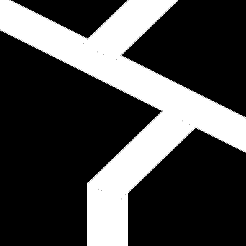
\includegraphics[width=0.35\textwidth]{complexFeatureApproach.png}
	\caption{An example of a complex approach to a feature which may undermine the current system feature detection.}
	\label{f:complexFeatureApproach}
\end{wrapfigure}

\section{Rotation of feature masks.} \textbf{TODO: Remove to appendix. }The current implementation has the system generating feature masks of the route feature as it will be approached and assumes a linear approach. This is a reasonable assumption for close in detection however it may fall down if complex approaches to route features are encountered. A more robust solution would involve developing the extended feature mask as outlined above and aligning the mask to the approach direction at the frame the feature will be detected. This would entail developing the mask as per section \ref{sect:route_feature_matching}-\ref{s:maskDevelopment} in the original paper and once developed, the mask can then be rotated so the approach line is vertical at the base of the image. On arrival at a feature node on the approach, the mask will be regenerated and reoriented. This approach takes advantage of the fact that the route between two nodes can be assumed as linear and will ensure the feature mask orientation will match the detected road more closely. 

An example of a complex approach to a feature is included as figure \ref{f:complexFeatureApproach}. In this instance as the vehicle encounters the first bend, the feature model mask will no longer have the correct orientation and result in a loss of feature tracking. 
	

\section{Navigation extension options.} While it was not explicitly considered as a feature, any road feature with a sharp enough angle between points can be used as a feature. This is particularly helpful if an aim is to identify a `true' position outside GPS error as bends in a road can be used as additional features without requiring additional intersecting roads. Additionally while this system was designed with a supporting GPS in mind to estimate anticipated feature arrival, as developed it does not rely on positional information specifically. Indeed assuming that relevant route feature data is stored, this system can work `offline' using the features as directions in a similar way a human navigator may. Integrating the output of this system with other sensors such as GPS offers additional localisation benefits. \citet{probabalisticRobotics} discuss Markov and extended Kalman filter localisation techniques that may be applicable to this system and have the potential to result in improved positional estimation.


\section{TODO}
Discuss Road detection mitigation (rolling average etc)
Add in references
	
\end{document}